\documentclass{article}
\usepackage[utf8]{inputenc}
\usepackage{graphicx}
\usepackage[
backend=biber,
style=authoryear,
citestyle=authoryear
]{biblatex}
\renewcommand*{\bibfont}{\small}
\usepackage[normalem]{ulem}
\usepackage{fancyhdr}
\usepackage{multicol}
\usepackage[hidelinks]{hyperref}
 
\pagestyle{fancy}
\fancyhf{}
\rhead{Can Meaning Travel?}
\lhead{Nicolai Berk}
\cfoot{\thepage}

\useunder{\uline}{\ul}{}

\addbibresource{PhD-Proposal.bib}


\usepackage{xcolor}

\title{Can Meaning Travel? The Causal Effect of Media Frames on Issue Definitions and Attitudes}
\author{Nicolai Berk\footnote{Doctoral Candidate, Dynamics Doctoral Program, Humboldt-Universität zu Berlin, \href{mailto:nicolai.berk@hu-berlin.de}{nicolai.berk@hu-berlin.de}}}
\date{May 2021}

\begin{document}

\maketitle

\begin{abstract}
    A large body of literature debates the existence and extent of effects of media framing on consumers' issue attitudes. At the same time, mechanisms of opinion formation have mainly been studied experimentally. Combining panel data from the German Longitudinal Election Study with fine-grained analyses of media framing, I address both debates with observational data. I provide strong evidence from 1,338 fixed-effect, difference-in-differences models suggesting the existence of media effects. Second, I show that such changes in consumers' issue attitudes do \textit{not} correspond to changes in the issue framing of their preferred media outlet. Instead, these changes could be explained by an ideological readership reacting differently to changes in the news agenda. Lastly, the study explores whether such changes in media framing affect consumers' issue definitions using state-of-the-art text analysis methods. The findings contribute to our understanding of opinion formation processes and the relevance of the news media in the 21st century.
\end{abstract}


\section{Introduction}

\begin{itemize}
  \item starting point: historical discussion on minimal vs maximal media effects and the discussion on external validity
  \item agenda setting yes (cite), but what about framing? Debate goes on
  \item second: unclear mechanisms - look for lab evidence to cite on this
\end{itemize}


\section{Framing in the wild}

\subsection{General evidence of framing effects}

argument 1: key issue is not the external validity of framing experiments, but the more likely to observe framing effects when consuming the SAME newspaper, which one trusts already - basically cue taking (Foos, Spirig, Ladd vs Gentzkow, Guess, resolved by Slothuus and Leeper)


\subsection{Mechanisms of framing}

argument 2: opinion shifts come about through changing associations (framing/issue definition) $\rightarrow$ value expectancy framework, but with a neurological basis


\subsection{Implications for the study of framing effects}
\begin{itemize}
\item Lesson: more observational data necessary, but we need to study cases where the slant of a newspaper that people already read changes, without obvious changes eg in ownership that made readers discount the slant
\item people could a) not care, b) stop reading their newspaper, c) change their opinion
\item changes in issue association should affect first people's issue definitions, which changes their opinion on the issue.
\end{itemize}

\section{Study design}

\subsection{Data and case description}

% plot with opinion development per paper for four / six issues

% plot with descriptives and survey dates

\subsection{Study design}

\subsubsection{Can framing effects among newspaper readers be observed?}

1,336 DiDs for all issue-paper-wave combinations

\subsubsection{Can these opinion shifts be explained by changing media frames?}

\begin{itemize}
    \item look at migration, maybe a second issue: how strongly do DiD's correlate with changing topic prevalence?
    \item look at how FE model DiD's change when controlling for newspaper attention/DiD
    \item add right/wing slant as second dependent using AfD-classifier
\end{itemize}


\subsubsection{Have readers' issue definitions changed as a result of the changing media frames?}

embedding regression: do shifts in migration definitions among the readers correspond to changes in the media definition?

\section{Results}

\subsection{DiD-assumption: Parallel trends}

% show graphs from issue with longest-running issues, add table with all graphs in appendix, show correlation of positions of different newspapers
\begin{figure}[!h]
    \centering
    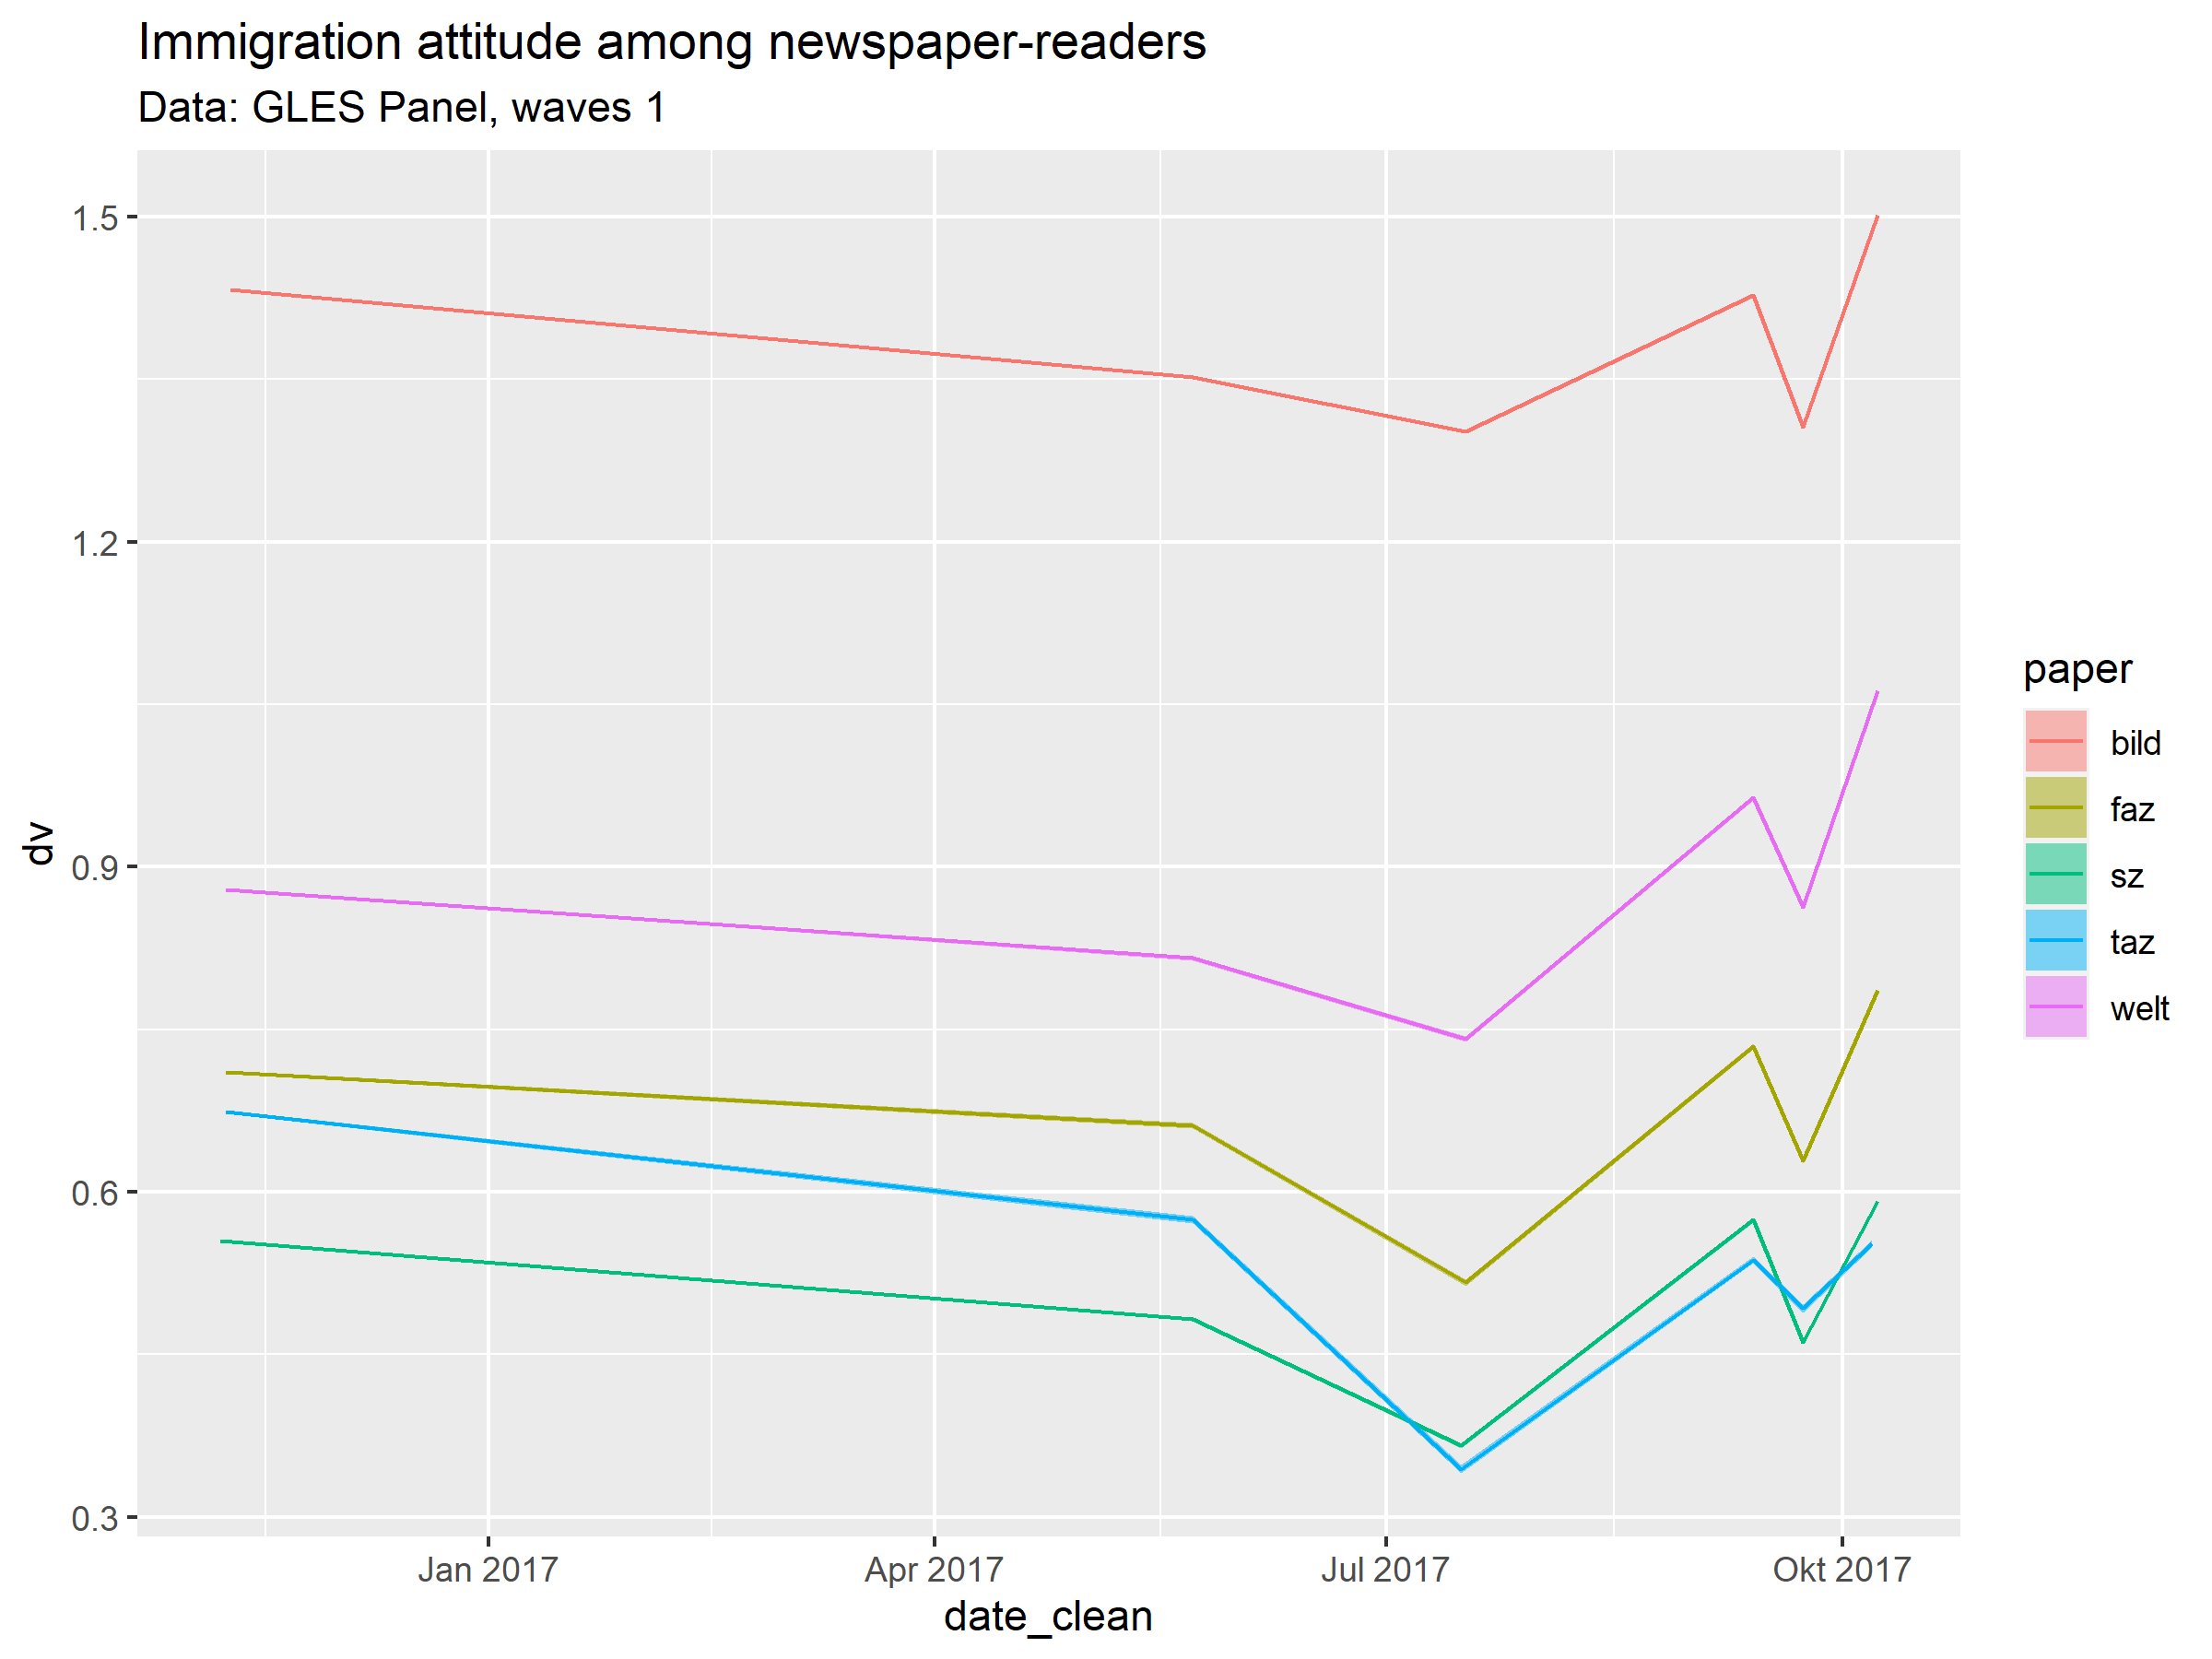
\includegraphics[width=\textwidth]{paper/vis/Immigration_papers.png}
    \caption{Opinions on migration across time, for different groups of readers.}
    \label{fig:issues}
\end{figure}
    
% also think about excludability: how can you ensure that these shifts are a result of media framing (this might be answered in number two)

\subsection{Distribution of DiD-effect significance}

% show distribution of p-values vs theoretical distribution -> looks like there is systematic deviation

\subsection{Correlation of DiD with frame prevalence}

% show correlation of DiD with prevalence of media frames (STM)

\subsection{Shifts in issue definitions}

% show for one specific case that shift in media frame corresponded to 

\section{Discussion}

\newpage

\section{Comments for Thomas}

Das hier war grob die geplante Vorgehensweise. Ich denke gegeben der Findings nicht so sinnvoll mehr, aber man könnte meines Erachtens in zwei Richtungen gehen: a) Evidenz zeigen, dass opinion shifts als Reaktionen ideologischer Leserschaft gelesen werden können (Modell mit Interaktion Migration attention und newspaper), b) Leserschaft als dependent, um zu zeigen, ob Framing shifts Leserschaft abstossen. Hier könnte man auch überlegen, ob das mit dem Slant der Zeitung zusammenhängt. Ausserdem könnte es auch re validity noch sinnvoll sein, wenigstens agenda-setting effects zu zeigen. Fraglich ist, ob es noch sinnvoll ist, die (methodisch eigentlich am spannendsten \& theoretisch an innovativsten) issue definitions zu analysieren. Eine nrecht einfache Erklärung für fehlende Effekte könnte auch fehlende Varianz, vor allem in den unabhängigen Variablen (Frames, Salienz) sein.

\end{document}